\chapter{简单理解计算机系统}

\begin{flushright}
本章节蒸馏自CMU与PKU的ICS课程,内容经过了大量的删减和改编,但尽可能地保留了原有的精华。
\end{flushright}

我在写第十章《用GDB调试》的时候,和LCPU的同学们在群聊里面吹了吹水。然后,我发现一个非常严重的问题:大多数人对于汇编、CPU、内存等概念都不甚了解,结果我写出来的一大堆东西全是鸡同鸭讲,堪比天书,这样的东西完全违背了我的本意。因此,我紧急中断了第十章的编写,决定先写一个mini ics,来介绍一下计算机的许多基本原理。

\textbf{我非常建议有时间的同学们阅读CSAPP这本经典教材,而且能读英文原版就读原版。}这是一本非常好的教材,内容非常全面,值得一读。我这一章是蒸馏版,把CSAPP的内容浓缩成了五个问题,并比原版教材更像“讲故事”,适合零基础的同学入门。当然,虽然说半小时就能看完、立刻就能用,但是毕竟是缺少了一大堆细节的。

\section{程序怎么跑起来?}

不知道同学们在写程序的时候,会不会疑惑“为什么我写的代码只是文本文件,但为什么这些特定的文本文件能够变成一个可以执行的程序、而我随便写的文章等却不能”。而另一个可能疑惑的问题是“只认识二进制的计算机,为什么能看懂我写的语言”。这就涉及到程序的编译和链接过程了。

我们知道,计算机的编程语言有很多种,这些高级语言都是方便人类来编写的。因此,就需要一些工具来把这些高级语言翻译成计算机能看懂的机器码(machine code)。对于C系语言写出的程序,一般情况下是由源代码(.c或.cpp文件)编译成目标代码(.o或.obj文件),然后链接成可执行文件(.exe或.out文件)。这个过程通常分为三个步骤:预处理、编译和链接。

\subsection{预处理}
预处理是对源代码进行一些简单的文本替换和宏展开。预处理器会处理一些指令,例如\texttt{\#include}、\texttt{\#define}等。同时,预处理会除去源代码中的所有注释。从某种程度上来说,预处理后的代码和源代码完全等价。

\subsection{编译和汇编}
计算机通过编译器将预处理后的代码转换为汇编码(能读懂一部分),然后再利用汇编器把汇编码转变成机器码(二进制码,人几乎读不懂)。编译器会将源代码转换为目标代码(.o或.obj文件),这个目标代码是特定于处理器架构的。这两步原理和过程相近,因此我们把它们合并在一起,但实际上是两步,这一点需要注意。

编译器会将源代码中的每个函数、变量等转换为机器码指令,并生成符号表(symbol table)来记录这些符号的地址。

编译器还会进行一些优化,例如常量折叠、循环展开等,以提高程序的执行效率。默认情况下,gcc编译器会进行一些基本的优化,但如果需要更高的优化级别,可以使用\texttt{-O2}或\texttt{-O3}选项。\textbf{优化可能暴露代码中的未定义行为},但是不会导致本符合标准的代码出现错误。因此,我们一定要尽可能地编写符合标准的代码。

\subsection{链接}
链接是将多个目标代码文件和库文件合并成一个基于特定操作系统的可执行文件的过程。链接器会将目标代码中的符号解析为实际的地址,并将它们合并成一个完整的可执行文件。链接也是一个比较复杂的过程,在这里我们不深入讨论。

\subsection{常见汇编码}

x86-64架构是Intel的64位架构,在现代计算机非常常见。我们会利用该架构来简单解释汇编码的语法。

在深入介绍汇编码之前,我们要先了解一下CPU的寄存器。寄存器是CPU内部的高速存储器,用于存储临时数据和指令。x86-64架构有16个通用寄存器(RAX、RBX、RCX、RDX、RSI、RDI、RBP、RSP、R8-R15),每个寄存器都是64位的。CPU将指令和数据加载到寄存器中,利用控制单元CU来执行指令,利用算术逻辑单元ALU来进行计算。

x86-64架构的汇编码通常由操作码(opcode)和操作数(operand)组成。操作码是指令的名称,操作数是指令的参数。以下是一些常见的汇编码指令:
\begin{itemize}
  \item \texttt{mov}:将数据从一个寄存器或内存位置移动到另一个寄存器或内存位置。
  \item \texttt{add}:将两个寄存器或内存位置的值相加,并将结果存储在第一个寄存器或内存位置中。
  \item \texttt{sub}:将一个寄存器或内存位置的值减去另一个寄存器或内存位置的值,并将结果存储在第一个寄存器或内存位置中。
  \item \texttt{jmp}:无条件跳转到指定的标签。
  \item \texttt{call}:调用函数,将返回地址压入栈中。
  \item \texttt{ret}:从函数返回,弹出栈顶的返回地址。
  \item \texttt{cmp}:比较两个寄存器或内存位置的值,并设置标志位。
  \item \texttt{je}、\texttt{jne}、\texttt{jg}、\texttt{jl}等:条件跳转指令,根据比较结果跳转到指定的标签。
\end{itemize}

在x86-64架构中,假如我们想要把某个整数从寄存器RAX移动到寄存器RBX,可以使用以下指令:
\begin{lstlisting}
mov rbx, rax
\end{lstlisting}
或者说我们想要call一个函数,假设函数名为\texttt{foo},可以使用以下指令:
\begin{lstlisting}
call foo
\end{lstlisting}
这是最基本的一些汇编码指令。对于其他的机器(例如Arm架构),汇编码的语法和指令可能会有所不同,但基本原理是相似的。编译器会在不同的架构上生成不同的汇编码,来保证程序的正确性和效率。

对于同一个机器,不同程序的同一句汇编码被编译出的机器码是一样的。比如说在x86-64架构上且使用AT\&T语法时,\texttt{mov rbx, rax}这句汇编码被编译成的机器码永远\texttt{48 89 D8},不会改变。

\subsection{其他情况}

对于解释性语言,情况略有不同。

以Python为例,它是一种解释性语言。这种语言并不需要先编译成机器码,而是通过解释器(例如CPython)先把\texttt{*.py}文件编译成\textbf{字节码}(bytecode)(.pyc文件),然后再由虚拟机(VM)来逐条解释执行这些字节码。字节码是一种中间表示形式,介于源代码和机器码之间。Python的字节码是与平台无关的,可以在任何支持Python解释器的系统上运行。而另一些工具(例如PyPy、Jython)会有JIT编译功能,能够把字节码编译成更高效的机器码来执行,而不是逐条解释执行。

而对于以C\#为首的“中间语言”,情况又略有区别。C\#是一种编译型语言,但它并不直接编译成机器码,而是编译成一种中间语言(Intermediate Language,IL),也叫做托管代码(Managed Code)。这种中间语言是一种与平台无关的字节码,可以在任何支持.NET框架的系统上运行。然后,.NET框架会利用即时编译器(JIT compiler)将中间语言编译成特定平台的机器码来执行。因此,C\#的逆向工程非常容易,直接反编译IL就能得到接近源代码的结果。

\subsection{从文件到程序}

刚才,我们知道了程序是怎么从源码转变成可执行文件的。那么,程序是怎么从可执行文件跑起来的呢?

在Linux中,可执行文件叫做ELF(Executable and Linkable Format)文件。ELF文件包含了程序的代码段(text segment)、数据段(data segment)、堆(heap)、栈(stack)等信息。操作系统通过加载器(loader)将ELF文件加载到内存中,并创建一个新的进程来执行该程序。在Windows中,可执行文件叫做PE(Portable Executable)文件,原理类似。

当我们运行一个可执行文件时,操作系统会将文件加载到内存中,并创建一个新的\textbf{进程}来执行该程序。每一个进程中都会有一个或多个\textbf{线程},线程是进程中的一个执行单元。每个线程都有自己的寄存器状态和栈空间,但多个线程可以共享进程的内存空间。
操作系统会为该进程分配内存空间,并将程序的代码和数据加载到内存中。然后,操作系统会将CPU的控制权转移到程序的入口点(通常是\texttt{main}函数),开始执行程序。

程序在执行过程中,CPU会不断地从内存中取指令,并执行这些指令。程序可能会调用其他函数、分配和释放内存、进行输入输出等操作。当程序执行完毕后,操作系统会回收该进程的资源,并将控制权返回给操作系统。一般情况下,程序只能够访问分配给自己的内存空间,不能访问其他进程的内存空间。程序一般无法直接操作外存中的内容,必须通过操作系统提供的系统调用来进行文件读写等操作,显著地降低了恶意程序破坏文件的风险。

当然,也有一些病毒等恶意程序会利用系统漏洞来直接操作其他进程的内存空间,或者直接操作外存中的内容,破坏文件系统的完整性和安全性。

\section{信息怎么被表示?}

我们写的程序中,有各种各样的数据类型,例如整数、浮点数、字符、字符串等。计算机也只认识0和1,那么,这些繁多的数据类型在计算机中是怎么被表示的呢?

在计算机上,信息是以二进制的形式被表示的,也就是0和1。每一个数字都是一个二进制位(bit),8个二进制位组成一个字节(byte)。于是我们就了解了:计算机上的数字只是约定好的0-1串,且要遵从一定的格式;计算机本身并不知道内存中这里存的是什么,这一切实际上都是程序告诉计算机的。于是你就理解了为什么在C系语言中的\texttt{union}可以把同一块内存当成不同类型来读写:内存中的0-1串并没有类型,类型只是程序员的约定。

为了表示方便,计算机上一般利用十六进制的两位来表示一个字节,例如十进制下的11,写成二进制是0b1011,写成十六进制是0xB;其中\texttt{0b}表示后面这个是二进制数\footnote{仅限于GNU语法},\texttt{0x}表示后面这个是16进制。有时候也可以看见这个数在八进制下的表示013,这个开头0就表示后面这个是8进制数。

\subsection{整数}
整数在计算机中通常使用补码的形式来表示。对于一个n位(这个n指的是二进制位)的有符号整数,最高位是符号位,其他n-1位用于表示数值;对于无符号整数,所有n位都用于表示数值。

例如一个四位的有符号整数,实际数值是各位数值相加,最高位表示$-2^3$,剩下的三位表示$2^2 + 2^1 + 2^0$,因此它的数值范围是$-8$(0b1000)到$7$(0b0111)。而一个四位的无符号整数,所有四位都表示数值,因此它的数值范围是$0$到$15$。

32位计算机中,常见的整数类型\texttt{int}指的通常是32位的整数(也就是4个字节)。于是我们就知道了,int类型的最大值是$2^{31}-1$,最小值是$-2^{31}$。而无符号整数类型\texttt{unsigned int}(以下简写为\texttt{uint})的最大值可以表示为$2^{32}-1$,最小值为0。在C/C++中,int的最大值有宏定义\texttt{INT\_MAX},最小值有宏定义\texttt{INT\_MIN},无符号整数的最大值有宏定义\texttt{UINT\_MAX}。

我们知道,十进制中的加法可能会产生进位。二进制加法也不例外,例如$1+1=10$。但是在刚刚的讲解中,我们发现对于\texttt{uint}类的变量,最长只有32位,那么如果两个变量相加,可能会超过32位,比如两个“1后面跟31个0”这样的整数相加,结果是1后面跟32个0,超过了32位,这个时候就会发生溢出(overflow)。我们一般不能依赖于溢出后的结果。

一般情况下,计算机对溢出行为的处理是取最低32位的结果。例如两个\texttt{uint}类型的变量相加,如果结果超过了32位,那么计算机往往会将结果的低32位作为最终结果返回。对于有符号整数(\texttt{int}),溢出结果按模$2^n$回绕;通常情况下也可以理解为将结果的低32位作为最终结果返回。(当然如果一开始就是两个更长的整数相加,例如两个64位的整数相加发生溢出时,就会返回低64位的结果。)

\subsection{浮点数}

浮点数是另一个表示实数的方式。浮点数在计算机中通常使用IEEE 754标准来表示。一个32位的浮点数(单精度)由三部分组成:符号位、指数位和尾数位。浮点数的本质是科学计数法的变种。
\begin{itemize}
  \item 符号位(1位):表示数值的正负。
  \item 指数位(8位):表示数值的指数部分。
  \item 尾数位(23位):表示数值的有效数字部分,存储的是隐含前导1的一个二进制小数,实际值是1.xxx。
\end{itemize}

具体说来,一个32位浮点数的数值可以表示为:
$$(-1)^{\text{符号位}} \times (1 + \text{尾数}) \times 2^{\text{指数} - 127}$$
其中,指数的偏移量是127,这个127的来源是$2^{(8-1)} - 1$。同理,一个64位的浮点数(双精度)由1位符号位、11位指数位和52位尾数位组成,指数的偏移量是1023。满足上述标准的单精度和双精度浮点数一般被称为规格化浮点数。因此,我们可以知道,最大的规格化单精度浮点数大概是$3.4 \times 10^{38}$,最小的规格化单精度浮点数大概是$1.2 \times 10^{-38}$;而最大的规格化双精度浮点数大概是$1.8 \times 10^{308}$,最小的规格化双精度浮点数大概是$2.2 \times 10^{-308}$。更精确的长数值(例如128位浮点数)也有类似的表示方法,这里就不赘述了。

现在的问题就变成,尾数位如果全是0,指数位如果全是0或者全是1,这种情况怎么办?IEEE 754标准对这些特殊情况做了规定:
\begin{itemize}
  \item 如果指数位全是0,尾数位全是0,那么表示的数值是0。
  \item 如果指数位全是0,尾数位不全是0,那么表示的数值是\textbf{非规格化数},用于表示非常接近0的数值。
  \item 如果指数位全是1,尾数位全是0,那么表示的数值是无穷大(Infinity)。
  \item 如果指数位全是1,尾数位不全是0,那么表示的数值是NaN(Not a Number),用于表示未定义或不可表示的数值,例如0除以0。
\end{itemize}
对于32位非规格化浮点数,数值可以表示为:
$$(-1)^{\text{符号位}} \times (0 + \text{尾数}) \times 2^{-126}$$
32位非规格化数的指数部分被固定为-126。同理,64位非规格化浮点数的指数部分被固定为-1022。因此最大的非规格化单精度浮点数大概是$1.7 \times 10^{-38}$,最小的非规格化单精度浮点数大概是$1.4 \times 10^{-45}$;而最大的非规格化双精度浮点数大概是$1.0 \times 10^{-307}$,最小的非规格化双精度浮点数大概是$5.0 \times 10^{-324}$。

然而,有些数值无法精确表示为二进制浮点数,例如十进制下的0.1在二进制下是一个无限循环小数,无法用有限的位数表示。因此,浮点数在计算机中往往只能\textbf{近似}表示某些实数,且在数非常大的时候精度会进一步降低。例如计算机实际上计算$0.1+0.2=0.3000\cdots 004$。另一方面,浮点数\textbf{并不连续},从上述表示方法可以看出浮点数也有间隔。一般的,把1到下一个浮点数之间的间隔叫做\textbf{机器精度},例如单精度浮点数的机器精度大概是$1.2 \times 10^{-7}$,双精度浮点数的机器精度大概是$2.2 \times 10^{-16}$。

另一方面,我们知道浮点数是科学记数法,其精度有限,在进行加法或乘法运算时不可避免地会导致舍入误差,而先丢失的精度可能会影响最终的结果,因此\textbf{浮点数的运算并不满足交换律和结合律}。例如$1.0 + 1.0 \times 10^{-7} - 1.0 \times 10^{-7} \neq 1.0 + (1.0 \times 10^{-7} - 1.0 \times 10^{-7})$。而在连续运算当中,这个舍入误差会累积,导致结果偏差越来越大。我们在实际操作中应当避免这种情况,例如可以将数值从小到大排序后再进行运算,并尽可能地减少数量级相差过大的数值运算,来减少累积误差。

作为Mini ICS,我们只需要知道浮点数有误差就可以了(这是因为十进制小数可能无法精确表示为二进制浮点数)。因此,工程上\textbf{不可以利用浮点数来进行货币运算},除非使用高精度浮点数(例如\texttt{decimal}类)。一般的处理是把货币放大100倍(也就是把元变成分),然后用整数来表示和计算。

有不少算法依赖于浮点数有精度这一客观事实,例如最大流算法中Ford-Fulkerson算法在计算机上的有限终止性证明就利用了这一特性。

\subsection{地址}

在内存中,每一个字节都有一个唯一的地址。地址通常是一个无符号整数,表示该字节在内存中的位置。地址的大小取决于计算机的架构,例如32位计算机的地址是32位的,而64位计算机的地址理论上是64位的(实际上大部分64位计算机只使用了48位或57位地址空间)。因此前者最多能表示4GB的内存,而后者理论上最多能表示16EB的内存。

有了地址,我们就可以对内存进行读写操作,也可以使用一些更高级的数据结构,例如数组、链表、树等。

\section{内存怎么被管理?}

刚刚我们提到,计算机的CPU从内存取指令和数据,执行指令,然后把结果再存回内存。但是现在的问题是:对于一些用户,我们可能会在后台挂着114514个进程,这些进程都需要使用内存。但是这些进程所占用的内存可能远远大于实际物理内存的大小。那么,计算机到底怎么管理内存,使得每个进程都能正常运行?

\subsection{虚拟内存}

计算机使用虚拟地址空间来管理内存。每个进程都有自己的虚拟地址空间,都认为自己是从0号地址开始用内存的。操作系统通过虚拟内存技术,将虚拟地址映射到物理地址。这样,每个进程都可以独立地使用内存,而不需要关心其他进程的内存使用情况。

打个比方:某高度智能运行的图书馆给每一本书贴一个标签,标签上写着书的编号;但是读者不需要管实际上书放在哪里,只需要知道自己的书编号就行了。

\subsection{磁盘交换区}

当物理内存不足时,操作系统会将一些不常用的页面(page)从物理内存(快)中换出到磁盘上的交换区(swap space)(慢)。我们可以理解为,图书馆把常用的书放在书架上,而不常用的书放在仓库里。这样,当需要使用不常用的书时,图书馆可以从仓库中取出书来。

\subsection{页面、页表、缺页异常}

页面是虚拟内存的基本单位,通常是4KB或8KB。操作系统使用页表(page table)来管理虚拟地址和物理地址之间的映射关系。如果我们查到了一个虚拟地址对应的物理地址,但是这个页面不在物理内存中,那么就会发生缺页异常(page fault)。操作系统会捕获这个异常,然后从磁盘上的交换区中加载相应的页面到物理内存中。同样利用图书馆打比方:图书馆有一本书的编号,但是这本书不在书架上,而是在仓库里。图书馆会去仓库里取出这本书,然后放到书架上。

如果最近的书架满了,怎么办呢?一个常见的策略是使用LRU(Least Recently Used)算法,淘汰最近最少使用的页面。也就是图书馆会把最近很久没被借阅的书从书架上拿下来,腾出空间来放新书。

\subsection{内存分配器}

内存分配器(memory allocator)是操作系统或运行时库提供的,用于管理进程的内存分配和释放。常见的内存分配器有\texttt{malloc}、\texttt{free}等函数。内存分配器会维护一张空闲内存块的列表,当进程请求分配内存时,分配器会从空闲列表中找到合适的内存块,并将其分配给进程。

假如我们在C系语言用了malloc函数分配了许多字节的内存,这时候操作系统\textbf{不会}直接分配物理内存,而是分配虚拟内存。操作系统会在页表中记录这个虚拟地址和物理地址的映射关系。而真正给物理页,是“用到才给”,多数情况下,当我们第一次访问这个虚拟地址时,操作系统会触发缺页异常,然后将对应的物理页加载到内存中;少数情况下(例如堆内存),操作系统会预先分配一些物理页而不是延迟到首次访问才分配。

这也可以解释为什么我malloc了10GB内存但是电脑依然流畅运行:还没真正分配呢。

\subsection{一个例子}

假如,我们打开了微信。这时候,操作系统给微信预留了1GB的虚拟地址空间;但是实际上只先分配很少数的物理内存来加载常用数据,剩下的全在磁盘交换区。然后,假设我们又切换到其他应用程序(例如去B站看视频),这时候B站会获得许多新的物理页,而微信的物理页会被换出去一部分。

现在老板给我发消息了,我打开微信,点击几下,这时操作系统触发一个缺页异常,然后微信数据又被拉回内存。如此反复,整个过程只在数十毫秒内完成,使得我们几乎感觉不到延迟。

因此以后谁再拿“某某手机/某某电脑真好,同时开十个APP也不卡”来宣传产品的时候,你可以跟他讲讲虚拟内存!

\section{怎么压榨CPU的性能?}

我们知道,CPU是计算机的核心部件,负责执行指令和处理数据,其做法是从内存中取指令和数据,执行指令,然后把结果再存回内存。但是,现在的计算机内存的速度已经远远跟不上CPU的速度了。我们怎么才能更进一步地压榨CPU的性能呢?

有时候在做超大矩阵乘法的时候,我们发现仅将循环从按列换成按行,或者从按行换成按列,就能将程序的运行速度提升许多。这又是为什么呢?这就涉及到了CPU的缓存机制。

\subsection{缓存的分级}

CPU的缓存(cache),又叫高速缓存,是一种小容量、高速度的存储器,用于存储经常使用的数据和指令。缓存通常分为三级:L1、L2和L3缓存。
\begin{itemize}
  \item L1缓存:位于CPU内部,速度最快(1纳秒级),但容量最小,通常为32KB或64KB。
  \item L2缓存:位于CPU内部或外部,速度较快(3到5纳秒级),容量较大,通常为256KB或512KB。
  \item L3缓存:位于CPU外部\footnote{现代CPU通常集成在内部做多核共享缓存},速度较慢(10纳秒级),但容量最大,通常为2MB或更大。
\end{itemize}
再往后就轮到内存了,内存的速度大约是100纳秒级别。我们可以利用小卖部来理解,L1缓存有点像学校每层楼都有的贩卖机,L2有点像每栋楼都有的小超市,L3有点像学校的大超市,而内存有点像学校外面的供货仓库。

\subsection{缓存行和局部性原理}

缓存是以缓存行为单位进行存储的。缓存行(cache line)是缓存中最小的传输单位,通常为64字节,但CPU依然能够按字节寻址。当CPU访问内存时,如果访问的地址在某个缓存行内,那么这个缓存行就会被加载到缓存中。我们可以这么理解:当我们去贩卖机只会买一瓶饮料,但是贩卖机补货的时候是一补补一箱。只要把经常一起用的数据放在连续的一个缓存行上,就能一口气全带走,非常方便。

缓存的局部性原理是指程序在执行过程中,访问数据的地址往往具有一定的规律性。局部性分为时间局部性和空间局部性。时间局部性指的是最近访问的数据很可能会再次被访问;空间局部性指的是如果访问了某个地址,那么很可能会访问相邻的地址。

因此,我们在编写程序时,应该尽量利用局部性原理,将相关的数据放在一起,减少缓存未命中(cache miss)的情况。

\subsection{组相联和标签}

缓存通常采用组相联(set-associative)方式来存储数据。组相联缓存将缓存分为多个组,每个组包含多个缓存行。当CPU访问某个地址时,首先计算出该地址对应的组,然后在该组内查找是否有对应的缓存行(way)。如果有,就命中(hit),否则就未命中(miss),需要从内存中加载数据。

每一个缓存行都会贴两个标签,一个是tag记录该缓存行对应的内存地址的高位部分,另一个是valid位记录该缓存行是否有效。在CPU要读一个地址的时候,CPU会先计算出该地址对应的组,然后在该组内查找是否有有效的缓存行。如果有,就命中;如果没有,就未命中,需要从内存中加载数据。

\subsection{未命中常见工作流程}

当CPU访问的地址不在缓存中时,就会发生读不命中。这时,CPU需要从内存中加载数据到缓存中。加载数据的过程通常分为以下几个步骤:
\begin{enumerate}
  \item L1缓存没有,去L2缓存查找;L2缓存没有,去L3缓存查找;L3缓存没有,去内存查找。
  \item 如果找到了,就将数据加载到L1缓存中,并更新L1缓存的标签和有效位。
  \item 如果L1缓存满了,就需要选择一个缓存行进行替换。通常使用LRU(Least Recently Used)算法来选择最近最少使用的缓存行进行替换。L2和L3缓存也会进行类似的替换操作。
\end{enumerate}

如果CPU试图往缓存中写入数据,而该缓存行已经被其他数据占用,那么就触发了写不命中。一般有一些策略来处理写不命中,例如写回(write-back)和直写(write-through)。写回策略是将数据先写入缓存,等到当缓存行被标记为“脏”时才写回时再写回内存;直写策略是直接将数据写入内存。写分配和不写分配是指在写不命中时,是否将数据加载到缓存中。写分配会将数据加载到缓存中,而不写分配则不会。

\subsection{大矩阵乘法的工作原理}
于是我们讲完了缓存,现在就可以来解释为什么有时候换个循环顺序就能提速一倍了。

一般情况下,一个二维数组,按行扫的时候,相邻的元素在内存连续,64个字节一口气全都搬进L1,命中率非常高;而按列扫的时候,相邻的元素在内存中并不连续,可能需要多次访问L2和L3缓存,命中率就会降低。

另一种方式就是手动对齐数据,例如利用结构体来对齐数据。这样可以防止诸如double等长数据类型被拆成好几个缓存行,手动对齐可以强制把这样的64位数据按进一个缓存行,速度至少翻倍。

简单地说,只要让常用数据挤在同一箱里,就能让小卖部永远有货。

\subsection{流水线}

上述缓存机制虽然显著提升了CPU的性能,但是CPU依然有一个瓶颈:指令执行的速度远远跟不上CPU的时钟频率\footnote{CPU的时钟频率指的是CPU每秒钟能够执行的时钟周期数,通常以GHz为单位表示。现代CPU的时钟频率通常在2GHz到5GHz之间,也就是每秒钟能够执行20亿到50亿个时钟周期。时钟周期是CPU时间的最小单位}。为了进一步提升CPU的性能,现代CPU采用了流水线(pipeline)技术。

这个流水线和工厂内的流水线非常类似。例如汽车组装工厂,现在并不是一辆车组装完了再组装下一辆车,而是把组装过程分成多个阶段,每个阶段由不同的工人负责。这样,当第一辆车进入第二个阶段时,第一辆车的第一个阶段已经完成,第二辆车可以进入第一个阶段进行组装。这样,工厂就能够同时组装多辆车,大大提高了生产效率。在CPU中,我们也是这样,把一个指令的执行过程分成:
\begin{enumerate}
\item \textbf{取指(IF)}:根据 PC 把指令读进指令寄存器;
\item \textbf{译码(ID)}:解析操作码、读寄存器堆拿到操作数;
\item \textbf{执行(EX)}:在 ALU 或地址生成单元里完成运算;
\item \textbf{访存(MEM)}:若是 load/store,访问数据缓存;
\item \textbf{写回(WB)}:把结果写回寄存器堆并更新标志位。
\end{enumerate}
然后和工厂中流水线一样,每一级都让独立的硬件单元完成。理想情况下,当上一条指令进入EX阶段时,下一条指令就跟着进入IF阶段,于是每个时钟周期都能完成一条指令的执行,大大提高了CPU的性能。

\begin{figure}[htbp]
  \centering
  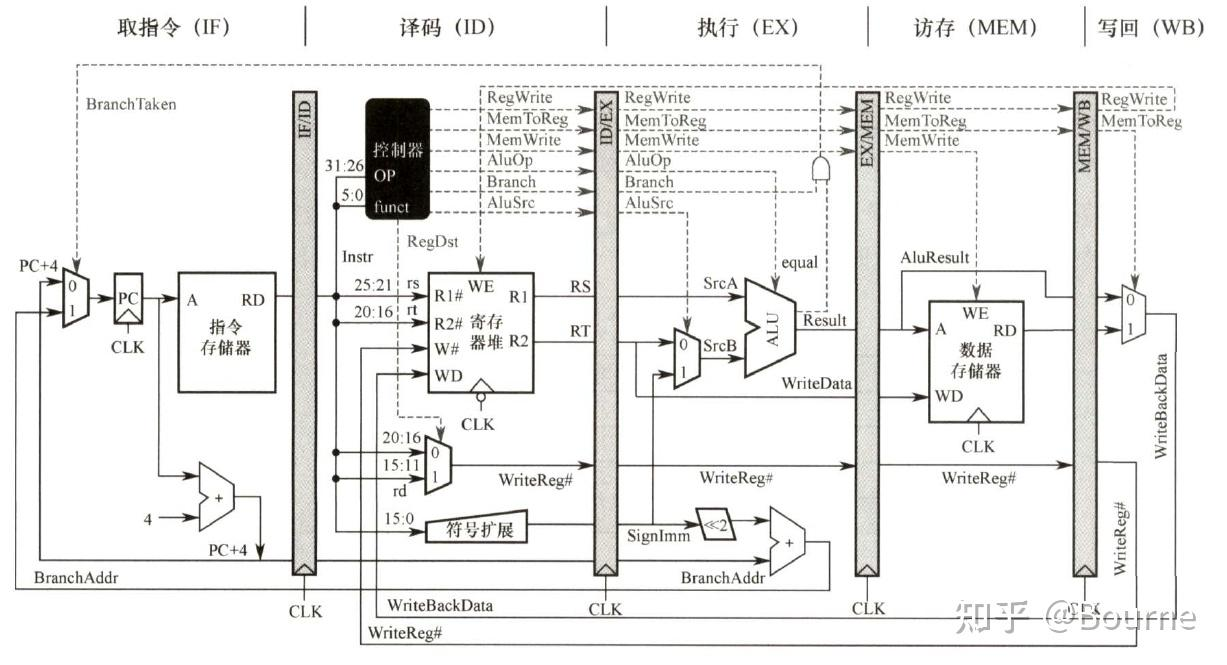
\includegraphics[width=0.8\textwidth]{106/pipeline.jpg}
  \caption{一张“臭名昭著”的流水线示意图}
\end{figure}

在实际情况下可能有三类“气泡”会让流水线停顿:
\begin{itemize}
  \item 数据冒险:当后一条指令恰好用到了前一条指令尚未写回的结果时,就会发生数据冒险,一个容易想到的解决方法是插入\textbf{气泡}(stall),让流水线停顿一段时间,直到前一条指令的结果写回。另外的解决方法是\textbf{数据转发}(或\textbf{数据前递},data forwarding),直接把前一条指令的结果旁路到后一条指令的EX级,避免停顿。
  \item 控制冒险:当遇到分支判断的时候,下一条指令的地址实际上是未知的。这时候也容易想到插入气泡来等待分支结果。为了防止这种情况,现代CPU通常会采用\textbf{分支预测}(branch prediction)技术,猜测下一条指令的地址,并提前加载到流水线中。如果猜测正确,就继续执行;如果猜测错误,就丢弃错误的指令,重新加载正确的指令,这样的代价是大约10到20个时钟周期的猜测惩罚。而怎么猜则是一个技术活,常见的方法有静态预测(例如总是猜测分支不跳转)和动态预测(例如利用历史信息来预测分支行为)。
  \item 结构冒险:当多个指令同时竞争同一个硬件资源时,就会发生结构冒险。例如,如果只有一个乘法器,而两条指令都需要使用乘法器,那么就会发生结构冒险。当然插入气泡也并非不可,而通过多端口寄存器堆、分离的指令和数据缓存等方法也可以缓解结构冒险的问题。
\end{itemize}

要是再往上提升性能,一般有三种手段:超标量(superscalar)、乱序执行(OoO)和超线程(SMT)。超标量指的是每一个周期同时发射多条指令到流水线中执行;乱序执行指的是指令不必严格按照程序顺序执行,而是可以根据数据依赖关系和资源可用性来动态调整执行顺序,只要操作数就绪了这条指令就可以抢跑,最后按指令序号重新提交结果;超线程指的是在流水线里面交替塞两条线程的指令,把闲置端口也利用起来。

以上操作对我们写代码有相当的启示:尽量保持分支可预测(有规律,少跳转),减少数据依赖(多用临时变量,少用全局变量),减少资源竞争(少用全局变量,少用锁),循环体小而整齐(减少指令数,增加指令并行度)。这样就能让流水线吃得饱饱的,性能自然就上去了。例如:
\begin{lstlisting}[language=C]
  int cnt = 0;
  for(int i = 0; i < n; i++)
    if (a[i] > 128)
      ++cnt
\end{lstlisting}
这个实践是不好的,因为数组模式随机,分支不可预测,数据依赖严重。改成下面这样就好多了:
\begin{lstlisting}[language=C]
  int cnt = 0;
  for(int i = 0; i < n; i++) {
    int flag = (a[i] > 128);
    cnt += flag;
  }
\end{lstlisting}
这样就消除了分支,数据依赖也减轻了许多,编译器大概会把上述内容编译成\texttt{setgt}和\texttt{add}指令,流水线就能更好地并行执行。

\begin{tip}
  当然,根据“不优化”原则我们知道,实际操作中未必需要严格这么写,或者说仅在以下情况差异显著:
\begin{itemize}
  \item 数据量巨大,例如n达到百万级别以上;
  \item 数据内容相当随机地分布,例如a[i]的值均匀分布在0到255之间;
  \item 编译器没有做激进优化,例如开的\texttt{-O0}或者\texttt{-O1};
  \item CPU是现代超标量、流水线深度相当大的CPU。
\end{itemize}
反之,当数据量小、大多数数据大于128(分支预测器能学习并预测)、编译器激进优化(“吸氧”甚至“吸臭氧”)、使用SIMD指令等技术时,差异就不明显了。

如希望验证我的上述说法,可以利用\texttt{perf}等工具进行性能分析,重点观察\texttt{branch-misses}、\texttt{instructions}、\texttt{cycles}等指标,\texttt{-O2}和\texttt{-O0}的差异也可以对比一下。
\end{tip}

\subsection{现代CPU的架构}

旧时代的CPU一般走的是单核高频路线,这也是非常容易想到的提升性能的方式:把一个核的频率提升到极限,然后让这个核尽可能地快地执行指令。这样做的好处是简单易行,缺点是功耗和发热量都非常高,且单核性能提升空间相当有限。这个路线撞墙的例子就是Intel的NetBurst架构(奔腾4),频率最高能达到3.8GHz,但是单核性能并没有显著提升,反而因为发热量过大而被迫降频。

于是,现代CPU性能渐渐地走向了多核化、并行化的路,性能不仅靠GHz撑着,并行度和专用加速也成为了重要的指标。当下主流芯片把多种计算单元拼成SoC,一般还有大小核之分(big.LITTLE架构),大核负责高性能计算,小核负责低功耗计算,二者协同工作以提升整体性能和能效比。

\begin{enumerate}
\item 性能核(P-core):乱序、宽发射、高频率,跑串行关键路径;
\item 能效核(E-core):顺序或窄发射,面积小、功耗低,跑后台线程;
\item 矢量/矩阵单元——SSE/AVX/AVX-512、SVE、AMX,一条指令打 512 bit–2048 bit 的 SIMD,做 dense math;
\item 集成 GPU Or NPU:上千线程级的 SIMT,负责图形与 AI 推理;
\item 片上系统:DDR/LPDDR 控制器、PCIe 5.0、CXL、缓存一致性总线(Ring/Mesh),把 CPU、GPU、加速器、内存、外设粘在一起。
\end{enumerate}

而缓存也从上文所述的经典缓存升级为支持网状多切片、非包容/非排他性、智能预取等特性的现代缓存系统,以适应多核、多线程、高并发的计算需求:

\begin{itemize}
\item 每个 P-core 独享 48 KB L1-I + 32 KB L1-D + 1–2 MB L2;
\item 多核通过 Mesh 节点共享 24–96 MB L3,切片数等于核数,降低热点;
\item 目录式(Directory)或总线嗅探(MESIF)协议保证多核一致性,跨核延迟 30–60 ns。
\end{itemize}

而对于我们开头的“超大矩阵乘法”这种还吃内存带宽的计算任务,现代CPU也有不少提升手段:

\begin{itemize}
\item AVX-512 / AMX:单指令可算 $16\times 64$ 矩阵块,理论算力提升4到8倍;
\item 高带宽内存:笔记本 LPDDR5X 已做到 120 GB/s,服务器 HBM3 突破 1 TB/s;
\item 缓存阻塞(cache blocking):把超大矩阵切成 L2 能装下的子块(如 $256 \times 256$),再在内层用 SIMD 展开,就能把 100 ns 的内存访问变成 5 ns 的 L2 命中,轻松获得10倍数级提速。
\end{itemize}

所以说,现代的CPU并不是单核跑分的时代,而是多核、矢量、缓存墙协同作战。写程序的时候,只需要让计算靠近数据、并行匹配硬件宽度,就能真正的把晶体管一滴不剩地榨成有效算力。

\section{系统怎么被调用?}

有时候我们电脑死机了,或者程序崩溃了,终端报错“Segmentation Fault”(段错误)。这时候,操作系统到底做了什么?为什么会发生段错误?我们来分析一下“系统调用”就知道了。

\subsection{为什么要有这个系统调用?}

一般情况下,程序运行时仅会访问分配给自身的内存中的数据和指令。如果程序试图访问未分配的内存区域,或者试图修改只读内存区域,就会发生段错误。这是出于安全性和稳定性的考量:操作系统需要确保每个进程都只能访问自己的内存区域,不能访问其他进程的内存区域。这样可以有效防止恶意程序破坏系统的稳定性和安全性。

但是有些情况下,程序确实需要访问一些特殊的内存区域,例如访问硬件设备、操作系统内核等。为了解决这种问题,操作系统提供了系统调用(system call)来处理内存访问。

简单地说,可以把操作系统看成化学实验室管理员,管理危化品。把危化品直接扔给学生非常危险,学生必须先向管理员填表申请,管理员检查后再给学生。填的这个表就是系统调用。

\subsection{系统调用长什么样?}

以Linux为例,一个系统调用往往包括系统调用号(放在RAX)、参数(放在RDI、RSI、RDX等寄存器,包括要干什么、干多少次、怎么干)、触发指令(\texttt{syscall})和返回值(放在RAX)。当程序需要进行系统调用时,会使用\texttt{syscall}指令来触发系统调用。系统调用的种类很多,例如read、write、open、close等,每个系统调用都有一个唯一的系统调用号。

以实验室为例,上述填表就包括:编号(系统调用号)、申请的危化品(参数)(包括要什么、要多少、放哪)、申请的指令(\texttt{syscall}),以及管理员的批复(返回值)。当学生需要使用危化品时,就会向管理员提交申请,管理员检查后返回批复。

\subsection{系统调用的处理流程}

当程序触发系统调用时,CPU会将当前的执行状态保存到内核栈中,然后切换到内核态(kernel mode)。在内核态下,操作系统会根据系统调用号找到对应的系统调用处理函数,并执行相应的操作。处理完成后,操作系统会将结果返回给用户态(user mode),并恢复之前保存的执行状态。

以\texttt{printf("Hello")}为例,这个东西实际上是做了一次系统调用\texttt{write(1, buf, 5)}。现在glibc把这玩意塞进寄存器触发syscall指令,然后CPU就切换到内核态。

之后,CPU在内核态办事:检查文件描述符1是否可写,发现可以写,就把Hello这5个字节写入到文件描述符1对应的设备(通常是终端)。

写完后,CPU会将结果(成功写入的字节数,在这里是5)放回RAX寄存器,然后切换回用户态。然后代码就会继续执行了。

\subsection{系统调用的代价与实践尝试}

系统调用虽然显著提升了系统的安全性,但是也带来了巨大的性能损失。因为每次系统调用都需要切换到内核态,这个过程需要保存和恢复CPU的状态,涉及到上下文切换(context switch),会消耗大量的时间,比普通函数调用慢不少——这还是现代CPU的优化结果。因此,系统调用的次数越少,程序的性能就越好。

在代码实践中,我们最简单的优化方式就是尽可能减少系统调用的次数,例如使用缓冲IO或批量读写等。

\begin{thinking}
  \begin{enumerate}
    \item 验证:浮点误差能累积到金融级别不可接受。试着使用不同的方法累加(不是乘法)1亿个0.01:\texttt{long double}、\texttt{double}、\texttt{float}、Kahan求和、\texttt{libmpdec}高精度库等,看看结果有什么差异。同时,使用\texttt{perf stat}等工具,看看不同方法的性能差异,量化误差和性能的权衡。最终,试着用文中提到的\texttt{int}方法来实现货币运算,看看结果和性能如何。
    \item 可执行文件究竟长什么样?GCC编译出的\texttt{*.o}和ELF文件究竟有什么差异?试着把这两个文件用十六进制编辑器打开,看看里面都有什么内容;标出ELF文件中的\texttt{e\_entry}、\texttt{program header}、\texttt{section header}等字段,并解释它们的作用。
    \item 优化究竟是怎么暴露未定义行为的?试着故意写一段有整数溢出的看似无害的UB代码,然后使用GCC编译器在不同的优化等级下编译,看看汇编码有什么差异(提示:用\texttt{diff}命令比较)。接着,试着打开UBSan运行程序,看看会发生什么。
    \item 虚拟内存真的是免费午餐吗?试着验证一下,当物理内存不足时,操作系统会将哪些页面换出到磁盘交换区?试着写一个程序,分配大量内存(例如\texttt{malloc 10GB})但不访问,观察VmSize和VmRSS的变化;然后,访问这些内存,观察VmSize和VmRSS的变化、记录SIGBUS或者真实缺页的次数,从而理解什么是overcommit(过度承诺)和OOM Killer,以及“用到才给”的含义。
    \item LRU真的永远是最优的吗?试着写一个程序,访问一个大数组(例如100MB),但是访问顺序是随机的,观察缓存命中率和程序运行时间。然后,试着改变访问顺序,例如按行访问、按列访问、斐波那契访问等,观察缓存命中率和程序运行时间的变化,从而理解局部性原理。另一方面,你能写一个程序,使得FIFO比LRU更优吗?
    \item 一条syscall指令事实上产生了多大的性能开销?试着写一个程序,频繁调用一个简单的系统调用(例如\texttt{getpid()}),然后使用\texttt{bpftrace}或者\texttt{perf}等工具,测量系统调用的延迟和CPU周期数,从而量化系统调用的开销。然后,试着将多个系统调用合并为一个系统调用(例如\texttt{io\_uring}),观察性能的提升,从而理解减少系统调用次数的重要性。
  \end{enumerate}
\end{thinking}
